% XCircuit output "HP.tex" for LaTeX input from HP.ps
\def\putbox#1#2#3#4{\makebox[0in][l]{\makebox[#1][l]{}\raisebox{\baselineskip}[0in][0in]{\raisebox{#2}[0in][0in]{\scalebox{#3}{#4}}}}}
\def\rightbox#1{\makebox[0in][r]{#1}}
\def\centbox#1{\makebox[0in]{#1}}
\def\topbox#1{\raisebox{-0.60\baselineskip}[0in][0in]{#1}}
\def\midbox#1{\raisebox{-0.20\baselineskip}[0in][0in]{#1}}
   \scalebox{1}{
   \normalsize
   \parbox{2.20312in}{
   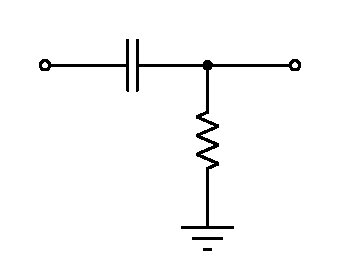
\includegraphics[scale=1]{HP}\\
   % translate x=447 y=332 scale 0.38
   \putbox{0.88in}{1.54in}{1.20}{\centbox{$C$}}%
   \putbox{1.47in}{0.79in}{1.20}{\midbox{$R$}}%
   \putbox{0.30in}{1.04in}{1.20}{\centbox{$V_{in}$}}%
   \putbox{1.97in}{1.04in}{1.20}{\centbox{$V_{out}$}}%
   } % close 'parbox'
   } % close 'scalebox'
   \vspace{-\baselineskip} % this is not necessary, but looks better
